\chapter{Implementation methodology}
As stated before we want to evaluate the perforamnce of CNN's to reconstruct images from compressed measurements. In this chapter we will describe the tools and software frameworks used in order to build the set-up for our experiments. First,  we introduce some of the most widly used libraries to build and train neural networks and the specific software tools for this thesis. Second, we briefly describe Graphics Processing Units (GPU's) and give reasons why they are an important tool when working with deep learning. Third, we will describe the datasets for training the networks and briefly justify its utilization. Then, we explain how the data is pre and postprocessed. This is important since it allows to efficiently use the hardware resources and makes the training process numerically stable. Finally, we propose CNN architectures for the reconstrution process.   

\section{Theano}
Theano is a library written in python that permits to define, optimize and compute mathematical expressions that deal with high-dimensional arrays in an efficient way. It is widly used among the deep learning community because it is optmized to make use of GPU routines that make training faster, efficient symbolic differentiation, stability optimizations and therefore making it realiable since it is constantly tested and debugged \cite{2016arXiv160502688short}. Nevertheless, Theano is not intendet to be used only for neural natwork applications. Therefore, it is necessary to write routines or API's that specially handle the difficulties encountered for deep learning. Such applications are normally an extra abstraction layer that sits on top of Theano's implementation and specially allow to build and train neural networks. Examples publically avaible are Lasagne \cite{sander_dieleman_2015_27878}, Blocks \cite{van2015blocks} and Keras \cite{chollet2015keras}. \\
Other common frameworks in deep learning are Google's Tensorflow \cite{tensorflow2015-whitepaper} that is written in C++, Torch \cite{torch} written in Lua and Caffe \cite{jia2014caffe} also written in C++. Most of them offer the same characteristics and mostly differ in the language they are written in, speed and target application, for example Caffe is not suitable for audio and text applciations.           
\subsection{Sdeepy}
Due to the fact that the previously mentioned implementations are constanly updated and changing, Sony decided to develop its own library to develop its projects. Sdeepy is an in-house Sony's deep learning library implmentation that makes used of Theano and incorporates routines commonly used as building-blocks for training and testing neural networks. It has the advantage that many new features can be added at any time they become available while maintaining the stability. Furthermore, it is easier to adapt and modify according to one's needs. Because of all that, we wil use Sdeepy for this thesis but, all implementations might be easily translated into any available framework.
\section{Graphics Procesing Unit (GPU)}
\begin{figure}[tb] 
\centering 
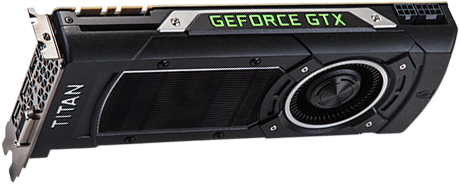
\includegraphics[scale=0.6]{GPU1.png} 
\caption[GPU for deep learning]{NVIDIA graphics card GeForce GTX Titan X used in our experiments.}
\label{fig:GPUim1} 
\end{figure}
A Graphics Processing Unit (GPU) is a chip architecture mainly desing for imaging and gaming. It differs from general-purpose CPU's in that they can handle larger amounts of data efficiently and faster in a parallel way, making them much more suitable for deep learning applications. It has extended its usage into machine learning area because companies like NVIDIA have develop GPU's specially optimized for neural networks. Not only that, but they have also written routines (NVIDIA Deep Learning SDK) that improve and speed up common operations like convolutions, better memory management and frienlier API's for easy learning. By distributing the workload of the training process the convergence happens much faster than  by using conventional CPU's. See Figure \ref{fig:GPUim1}
\section{Datasets}
It is also important to mention that along with better hardware and more ingenious algorithms deep learning has achieved major sucess because in recent years more and more data is becoming available through the internet. For most of machine learning methods data is the most important asset to obtain sucessfult results. In fact, choosing the right dataset is the first step in the deep learning workflow cycle and it is, in general, much more important than the chosen learning algorithm itself. \\
Since our goal is to reconstruct images, we make use of three different image datasets BioID \cite{frischholz2003bioid}, Label faces in the wild (LFW) \cite{LFWTech} and LabelMe \cite{russell2008labelme}. The first two datasets served as an initial baseline for measuring the plausibility of our approach and the last one allows for a more robust justification as explained later. All of the datasets are known in the community for being applied for different tasks like face detection, emotion recognition and image classification. Here, we propose its usage for image reconstruction from compressed samples. \\
\begin{table}[tb]
\caption[Datasets for training and testing]{Original features of each dataset.}
\label{tab:datasets1}
\centering
\begin{tabular}{l*{6}{c}r}
Dataset name              & Number of images & training & testing &  Original image size& Grayscale \\
\hline
BioID   & 1521 & 1371 & 150 & 384x286 & Yes\\
LFW     & 13233 & 11933 & 1300 & 250x250 & No\\
LabelMe & 50000 & 40000 & 10000 & 256x256 & No\\
\bottomrule 
\end{tabular}  
\end{table}

All datasets differ in terms of image size, color model (RGB or Grayscale) and file format (jpg, png, bmp, etc.). In order to facilitate implementation all datasets had to be transformed into a more generic form that could meet our constrains. Namely, it is more convenient to work with grayscale images and once promissing result are obtained it can be easily extend to RGB imgaes or even video. For that reason LFW and LabelMe datasets were converted into grayscale images using rgb2gray MATLAB function. Furtheremore, having an image size that was divisible by 16 was an initial requirement and so each image was resize to $256x256$ using imresize. The actual data being used is described in table \ref{tab:datasets2}.   
\begin{table}[tb]
\caption[Transformed datasets for training and testing]{Transformed features of each dataset.}
\label{tab:datasets2}
\centering
\begin{tabular}{l*{6}{c}r}
Dataset name              & Number of images & training & testing &  Original image size& Grayscale \\
\hline
BioID   & 1521 & 1371 & 150 & 256x256 & Yes\\
LFW     & 13233 & 11933 & 1300 & 256x256 & Yes\\
LabelMe & 50000 & 40000 & 10000 & 256x256 & Yes\\
\bottomrule 
\end{tabular}  
\end{table}

Finally in order to evaluate the performance of our trained network we introduce a set of 18 images. The images, we believe, are the most popular ones in the image processing community and serve as a baseline for many reconstruction algorithms and image processing tasks. They also help compared our results against the ones reported by other researchers. The evaluation set is shown in figure \ref{fig:EVALim1}
\begin{figure}[tb] 
\centering 
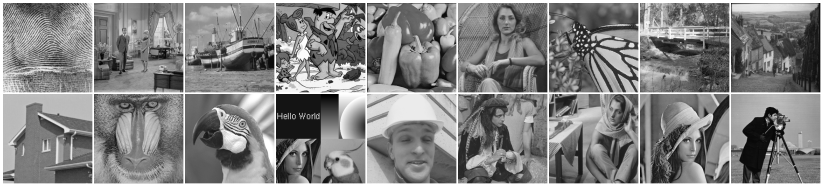
\includegraphics[scale=0.7]{EVAL1.png} 
\caption[Evaluation images]{From Top Left to Right Bottom:'fingerprint','couple','boats','flintstones','peppers','woman',
'butterfly','bridge','houses','house','mandril','parrot','montage','foreman','man','barbara','lena','cameraman'}
\label{fig:EVALim1} 
\end{figure}